% !TEX encoding = UTF-8 Unicode
%----------------------------------------------------------------------------------------
% Some of the standard documentclass types are:
% article --- for articles in journals, short reports, documentation, invitations etc...
% proc --- class for proceedings based on article class
% report --- for longer reports with several chapters, small books, thesis
% book --- for real books
% letter --- for writing letters
% beamer --- for writing presentations

% Some of the frequently used optional parameters:
% 10pt (default), 11pt, 12pt --- font size
% a4paper (default), letterpaper, a5paper etc --- paper size
% draft --- disables figures and is used to speed up typesetting during development
% onecolumn (default), twocolumn --- text layout
% fleqn --- left alignment of formulas
% leqno --- labels formulas on the left-hand side (instead of right)
% landscape --- use landscape page layout
% oneside (default for article and report), twoside (default for book)
% notitlepage (default for article), titlepage (default for report and book) --- display title page
% openany (default for report), openright (default for book) --- open chapters on any page, or only on odd pages

\documentclass[12pt,twoside,a4paper]{article}

%----------------------------------------------------------------------------------------
% The package provides an easy and flexible user interface to customize page layout,
% implementing auto-centering and auto-balancing mechanisms so that the users have only
% to give the least description for the page layout.
\usepackage[margin=10mm]{geometry}
% Introduces command \newgeometry{left=10mm,right=30mm,top=20mm,bottom=20mm},
% that can be used to change margins in the middle of the document.

%----------------------------------------------------------------------------------------
% Fontspec is a package for XeLaTeX and LuaLaTeX.
% It provides an automatic and unified interface to feature-rich AAT and OpenType fonts
% through the NFSS in LaTeX running on XeTeX or LuaTeX engines.
\usepackage{fontspec}

% Windows standard fonts with cyrillic support:
%\setmainfont{Times New Roman}
%\setsansfont{Arial}
%\setmonofont{Latin Modern Mono}

% Linux standard fonts with cyrillic support:
\setmainfont{Liberation Serif}
\setsansfont{Liberation Sans}
\setmonofont{Liberation Mono}

%----------------------------------------------------------------------------------------
% Alternative: babel package
% This package manages culturally-determined typographical (and other) rules
% for a wide range of languages. A document may select a single language to be supported,
% or it may select several, in which case the document may switch
% from one language to another in a variety of ways.
%\usepackage{polyglossia}
%\setmainlanguage{russian}
%\setotherlanguage{english}
% Note, that since polyglossia hardly relies on fontspec package,
% defined above fonts should support chosen language.
% Otherwise you will get a polyglossia error.

% Use \selectlanguage{<language>} to switch between languages, and
% \foreignlanguage{<language>}{<text>} to write text on specified language.
% Define auxiliary commands to switch languages.
%\newcommand{\ru}[1]{\foreignlanguage{russian}{#1}}
%\newcommand{\en}[1]{\foreignlanguage{english}{#1}}

%----------------------------------------------------------------------------------------
% Alternative: polyglossia package
% This package manages culturally-determined typographical (and other) rules
% for a wide range of languages. A document may select a single language to be supported,
% or it may select several, in which case the document may switch
% from one language to another in a variety of ways.
\usepackage[main=russian,english]{babel}
% Note, that since babel hardly relies on font configuration,
% defined above fonts should support chosen language.
% Otherwise you will get a polyglossia error.

% Use \selectlanguage{<language>} to switch between languages, and
% \foreignlanguage{<language>}{<text>} to write text on specified language.
% Define auxiliary commands to switch languages.
\newcommand{\ru}[1]{\foreignlanguage{russian}{#1}}
\newcommand{\en}[1]{\foreignlanguage{english}{#1}}

%----------------------------------------------------------------------------------------
% Bibliography package
\usepackage[
  backend=biber,       % use biber to process .bib files
  style=gost-numeric,  % ГОСТ 7.1 --- 2003
  autolang=other,
  isbn=true,
  url=false
]{biblatex}

\renewcommand*{\mkbibhdnamefamily}[1]{#1}  % disable italic text in author field

% Specify files (list of comma separated values) containing bibliography database
\addbibresource{bibliography.bib}

%----------------------------------------------------------------------------------------
% The tocloft package provides means of controlling the typographic design
% of theatricalisation Table of Contents, List of Figures and List of Tables. 
\usepackage{tocloft}

%\renewcommand{\cftpartleader}{\cftdotfill{\cftdotsep}} % add dots for parts
%\renewcommand{\cftchapleader}{\cftdotfill{\cftdotsep}} % add dots for chapters
\renewcommand{\cftsecleader}{\cftdotfill{\cftdotsep}} % add dots for sections

% Set equal indents for all toc entries
%\cftsetindents{section}{0em}{2em}
%\cftsetindents{subsection}{0em}{2em}

%----------------------------------------------------------------------------------------
\usepackage{amsmath,amsthm,amssymb}  % math packages
\usepackage{dsfont}  % math font

%----------------------------------------------------------------------------------------
% The caption package provides many ways to customise the captions in floating environments
% like figure and table, and cooperates with many other packages
\usepackage{caption}

%----------------------------------------------------------------------------------------
% This package provides advanced facilities for inline and display quotations.
% Recommended for use with babel/polyglossia
\usepackage{csquotes}
% Introduces commands:
% \blockquote[<cite>][<punct>]{<text>} --- quote text
% \hyphenblockquote[<cite>][<punct>]{<text>} --- quote text on a foreign language

%----------------------------------------------------------------------------------------
% The package provides extensive facilities, both for constructing headers and footers,
% and for controlling their use.
\usepackage{fancyhdr}

% Add link to table of contents at the footer of each page
\pagestyle{fancy}
\renewcommand{\headrulewidth}{0pt}% removes header line
\fancypagestyle{plain}{% for chapter starting pages
  \fancyhf{}% clears header fields
  \cfoot{\hyperlink{contents}{\contentsname}\hfill\thepage}}
% links the TOC at the center of the page footer
\cfoot{\hyperlink{contents}{\contentsname}\hfill\thepage}

%----------------------------------------------------------------------------------------
% This package prevents page numbers and headings from appearing on empty pages. 
\usepackage{emptypage}

%----------------------------------------------------------------------------------------
% The appendix package provides various ways of formatting the titles of appendices. 
\usepackage{appendix}

%----------------------------------------------------------------------------------------
% The verbatim package reimplements the LaTeX verbatim and verbatim* environments.
% The package also provides a comment environment (that skips everything between
% \begin{comment} and \end{comment}), and a command \verbatiminput for typesetting
% the contents of a file, verbatim.
\usepackage{verbatim}

%----------------------------------------------------------------------------------------
% The package was designed to accommodate all needs for inclusion of graphics in LaTeX documents
\usepackage{graphicx}

% Declare paths to graphics and extensions
\graphicspath{{./pictures/}{./plots/eps}}
\DeclareGraphicsExtensions{.pdf,.jpeg,.png,.eps}

%----------------------------------------------------------------------------------------
% epstopdf is a Perl script that converts an EPS file to an 'encapsulated' PDF file
\usepackage{epstopdf}
\epstopdfsetup{outdir=./build/}  % set output directory for auxiliary files
\epstopdfsetup{update}  % only regenerate pdf files when eps file is newer

%----------------------------------------------------------------------------------------
% The color package provides both foreground (text, rules, etc.) and background colour management
% Relies on graphicx package
\usepackage{xcolor}

%----------------------------------------------------------------------------------------
% An extended implementation of the array and tabular environments which extends the options for column formats,
% and provides "programmable" format specifications.
\usepackage{array}

%----------------------------------------------------------------------------------------
% These packages offer a series of extensions to the standard tabular environment:
% multirow provides a construction for table cells that span more than one row of the table;
% bigstrut creates struts which (slightly) stretch the table row in which they sit;
% bigdelim creates an appropriately-sized delimiter (for example, brace, parenthesis or bracket)
% to fit in a single multirow, to indicate a relationship between other rows
\usepackage{multirow}

%----------------------------------------------------------------------------------------
% The package enhances the quality of tables in LaTeX, providing extra commands
% as well as behind-the-scenes optimisation.
% Allows the use of \toprule, \midrule and \bottomrule commands in tables.
\usepackage{booktabs}

%----------------------------------------------------------------------------------------
% Provides support for the manipulation and reference of small or ‘sub’ figures and tables
% within a single figure or table environment
\usepackage[font=normalsize,labelfont=sf,textfont=sf]{subfig}

%----------------------------------------------------------------------------------------
% Multicol defines a multicols environment which typesets text in multiple columns
% (up to a maximum of 10), and (by default) balances the end of each column at the end of the environment.
% To adjust column contents more precisely use minipage environment.
\usepackage{multicol}

%----------------------------------------------------------------------------------------
% The hyperref package is used to handle cross-referencing
% commands in LaTeX to produce hypertext links in the document.
\usepackage{hyperref}

% Define color scheme of links (xcolor package is required)
\hypersetup{
  unicode,
  colorlinks,
  citecolor=red,
  filecolor=black,
  linkcolor=red,
  urlcolor=red
}

%----------------------------------------------------------------------------------------
% The command \url is a form of verbatim command that allows linebreaks at certain
% characters or combinations of characters, accepts reconfiguration,
% and can usually be used in the argument to another command.
\usepackage{url}
\urlstyle{same}  % use current text font for url links

%----------------------------------------------------------------------------------------
% The package enables the user to typeset programs (programming code) within LaTeX;
% the source code is read directly by TeX --- no frontend processor is needed.
\usepackage{listings}

% Define styles for C++ listings
\definecolor{dkgreen}{rgb}{0,0.6,0}
\definecolor{gray}{rgb}{0.5,0.5,0.5}
\definecolor{mauve}{rgb}{0.58,0,0.82}

\lstset{frame=tb,
  language=C++,
  aboveskip=3mm,
  belowskip=3mm,
  showstringspaces=false,
  columns=flexible,
  basicstyle={\small\ttfamily},
  numbers=left,
  numberstyle=\tiny\color{gray},
  keywordstyle=\color{blue},
  commentstyle=\color{dkgreen},
  stringstyle=\color{mauve},
  breaklines=true,
  breakatwhitespace=true,
  tabsize=3,
  xleftmargin=0.5cm,
  frame=lr,
  framesep=8pt,
  framerule=0pt,
  otherkeywords={*,__m256i}
}

%----------------------------------------------------------------------------------------
% Algorithm2e provides an environment for writing algorithms
\usepackage[ruled,lined,noend,linesnumbered]{algorithm2e}

%----------------------------------------------------------------------------------------
% PGF is a macro package for creating graphics
\usepackage{tikz}
%\usepackage{pgffor}
%\usepackage{ifthen}
%\usepackage{animate}

%----------------------------------------------------------------------------------------
% This package provides \todo{} command, that places visual notifications in text
% use [disable] option to remove all todoes from text
\usepackage[colorinlistoftodos,prependcaption,textsize=tiny]{todonotes}

\setlength{\marginparwidth}{2cm}  % set width of margin where comment will be placed

%----------------------------------------------------------------------------------------
%       GLOBAL CONFIGURATION AND DEFINITIONS
%----------------------------------------------------------------------------------------
% Declare math operators such as \min or \arg that will be used in math formulas
\DeclareMathOperator{\argmax}{argmax}
\DeclareMathOperator{\diag}{diag}
\DeclareMathOperator{\GF}{GF}
\DeclareMathOperator{\sgn}{sgn}
\DeclareMathOperator{\wt}{wt}

%----------------------------------------------------------------------------------------
\newtheorem{mdefinition}{Определение}
\newtheorem{mtheorem}{Теорема}
\newtheorem{mexample}{Пример}

%----------------------------------------------------------------------------------------
%       CUSTOM COMMANDS
%----------------------------------------------------------------------------------------
% Define shortcuts
\newcommand\mbA{\mathbb{A}} \newcommand\mbB{\mathbb{B}}
\newcommand\mbC{\mathbb{C}} \newcommand\mbD{\mathbb{D}}
\newcommand\mbE{\mathbb{E}} \newcommand\mbF{\mathbb{F}}
\newcommand\mbG{\mathbb{G}} \newcommand\mbH{\mathbb{H}}
\newcommand\mbI{\mathbb{I}} \newcommand\mbJ{\mathbb{J}}
\newcommand\mbK{\mathbb{K}} \newcommand\mbL{\mathbb{L}}
\newcommand\mbM{\mathbb{M}} \newcommand\mbN{\mathbb{N}}
\newcommand\mbO{\mathbb{0}} \newcommand\mbP{\mathbb{P}}
\newcommand\mbQ{\mathbb{Q}} \newcommand\mbR{\mathbb{R}}
\newcommand\mbS{\mathbb{S}} \newcommand\mbT{\mathbb{T}}
\newcommand\mbV{\mathbb{V}} \newcommand\mbU{\mathbb{U}}
\newcommand\mbW{\mathbb{W}} \newcommand\mbX{\mathbb{X}}
\newcommand\mbY{\mathbb{Y}} \newcommand\mbZ{\mathbb{Z}}

\newcommand\mcA{\mathcal{A}} \newcommand\mcB{\mathcal{B}}
\newcommand\mcC{\mathcal{C}} \newcommand\mcD{\mathcal{D}}
\newcommand\mcE{\mathcal{E}} \newcommand\mcF{\mathcal{F}}
\newcommand\mcG{\mathcal{G}} \newcommand\mcH{\mathcal{H}}
\newcommand\mcI{\mathcal{I}} \newcommand\mcJ{\mathcal{J}}
\newcommand\mcK{\mathcal{K}} \newcommand\mcL{\mathcal{L}}
\newcommand\mcM{\mathcal{M}} \newcommand\mcN{\mathcal{N}}
\newcommand\mcO{\mathcal{0}} \newcommand\mcP{\mathcal{P}}
\newcommand\mcQ{\mathcal{Q}} \newcommand\mcR{\mathcal{R}}
\newcommand\mcS{\mathcal{S}} \newcommand\mcT{\mathcal{T}}
\newcommand\mcV{\mathcal{V}} \newcommand\mcU{\mathcal{U}}
\newcommand\mcW{\mathcal{W}} \newcommand\mcX{\mathcal{X}}
\newcommand\mcY{\mathcal{Y}} \newcommand\mcZ{\mathcal{Z}}

%----------------------------------------------------------------------------------------
% \newcommand* cannot contain \par
\newcommand*\norm[1]{\left\lVert#1\right\rVert}
\newcommand*\set[1]{\{#1\}}
\newcommand*\tuple[1]{\langle #1 \rangle}

% put text into a circle
\newcommand*\circled[1]{\tikz[baseline=(char.base)]{
            \node[shape=circle,draw,inner sep=2pt] (char) {#1};}}
% put text in a square
\newcommand*\squared[1]{\tikz[baseline=(char.base)]{
            \node[shape=rectangle,draw,inner sep=3pt] (char) {#1};}}

%----------------------------------------------------------------------------------------
%       DOCUMENT
%----------------------------------------------------------------------------------------
%----------------------------------------------------------------------------------------
\begin{document}
% This declaration makes TeX less fussy about line breaking.
% This can prevent overfull boxes, but may leave too much space between words.
\sloppy
\pagenumbering{gobble}  % remove page numbers (and reset to 1)
\clearpage

%----------------------------------------------------------------------------------------
%       TITLE SECTION
%----------------------------------------------------------------------------------------
% Place title on the separate page
% maketitle
\title{Шаблон документа для LuaLaTeX}
\author{Николай Якуба\\nick.yakuba@gmail.com}
\date{2018}

\maketitle
\thispagestyle{empty}  % remove any header and footer (including page number)

%----------------------------------------------------------------------------------------
% titlepage
\begin{titlepage}
  \begin{center}
    Министерство образования и науки Российской Федерации\\
    Санкт-Петербургский политехнический университет Петра Великого\\
    Высшая школа программной инженерии\\
  \end{center}
  \vspace{0.3\textheight}

  \begin{center}
    {\Huge Название работы}\\
    \vspace{0.05\textheight}
    \begin{tabular}{lll}
      & \hspace*{0.3\textwidth} & \\
      Выполнил & & \\
      студент гр. 12345& &Н.В. Якуба\\[0.5em]
      Руководитель & & \\
      к.т.н, доцент & & П.В. Трифонов\\
    \end{tabular}
    \vfill
    Санкт-Петербург\\
    \the\year 
  \end{center}
\end{titlepage}


%----------------------------------------------------------------------------------------
\cleardoublepage  % start actual document from the odd page
\newgeometry{left=10mm,right=30mm,top=20mm,bottom=20mm}  % set page margins

\pagestyle{plain}  % restore default footer with page number
\pagenumbering{arabic}  % restore page numbers (alatexnd reset to 1)
\setcounter{page}{2}  % set first page number = 2

%----------------------------------------------------------------------------------------
%       ABSTRACT
%----------------------------------------------------------------------------------------
\begin{abstract}
  Данный документ является шаблоном, который может быть использован для создания отчетов, статей и других документов.

  Файл {\em main.tex} содержит общие настройки шаблона, а также список используемых пакетов.
  Файл {\em title.tex} используется для описания титульного листа.
  Текст документа, тестирующий возможности используемых расширений, находится в файле {\em document.tex}.
\end{abstract}

%----------------------------------------------------------------------------------------
%       TABLE OF CONTENTS
%----------------------------------------------------------------------------------------
\setcounter{tocdepth}{3}  % use at most 3 levels in table of contents
\hypertarget{contents}{}  % set anchor for link to contents from footer
\tableofcontents
\clearpage

%----------------------------------------------------------------------------------------
%       BODY OF THE DOCUMENT
%----------------------------------------------------------------------------------------
\section{Введение}
TeX --- это система компьютерной верстки, разработанная американским профессором информатики Дональдом Кнутом в 1978.
Вместе с языком описания шрифтов Metafont TeX был предназначен для быстрого создания документов высокого качества, а также для предоставления инструментов, дающих одинаковый результат на всех компьютерах.

LaTeX является надстройкой над TeX, включающей в себя огромное число макросов и расширений, упрощающих создание документов.
LuaLaTeX в свою очередь расширяет возможности LaTeX, предоставляя поддержку unicode и интегрируя язык Lua для создания сложных расширений.

%----------------------------------------------------------------------------------------
\subsection{Hello, world!}
Самый базовый документ приведен на рисунке \ref{f1}.
Документ начинается с указания его типа.
В данном случае это {\em article}.
Текст документа должен быть заключен между {\textbackslash}begin\{document\} и {\textbackslash}end\{document\}.
Число пробелов в строке не влияет на ее отображение.

\begin{figure}[b]  % display figure in the [b]ottom of the page
  \centering
\begin{verbatim}
\documentclass{article}
\begin{document}
This is my \emph{first} document prepared in \LaTeX.
\end{document}
\end{verbatim}
\caption{Пример документа}
\label{f1}
\end{figure}

Текст разделяется на абзацы.
Для перевода текста на новую строку можно использовать макрос '{\textbackslash}{\textbackslash}'.
Ниже слева приведен код TeX, а справа --- его отображение в документе.
\begin{multicols}{2}
\begin{verbatim}
Дефис: какой-то.

Новый абзац.\\
Перенос. Интервал 10 -- 15.

Это предложение --- текст,
в котором есть тире.
\end{verbatim}
  \columnbreak
Дефис: какой-то.

Интервал 5 -- 10.\\
Интервал 10 -- 15.

Это предложение --- текст,
в котором есть тире.
\end{multicols}

Более подробное введение можно прочитать в \cite{latexWikibook}.

%----------------------------------------------------------------------------------------
\section{Возможности TeX}
\subsection{Титульный лист и оглавление}
Существует несколько способов сформировать титульный лист.
Первый способ --- использовать команду '{\textbackslash}maketitle'.
Перед ее вызовом необходимо указать название работы, перечислить авторов, а также указать дату.

Второй способ заключается в создании отдельной страницы.
Для ее создания используется окружение {\em titlepage}.

Для создания оглавления используется команда '{\textbackslash}tableofcontents'.

Подробнее см. \cite{latexTitle,latexTOC}

%----------------------------------------------------------------------------------------
\subsection{Списки}
Существует 2 типа списков:
\begin{enumerate}
\item Нумерованный список (окружение {\em enumerate})
\item \label{item2}
  Ненумерованный список (окружение {\em itemize})
\end{enumerate}

Каждый элемент списка начинается с команды '{\textbackslash}item', нумерация осуществляется автоматически.
На элементы списка можно ссылаться.
Ниже приведен пример списка \ref{item2}.

\begin{itemize}
\item первый тезис
\item второй тезис
\item третий тезис
\end{itemize}

Подробнее о списках можно прочитать в документации \cite{latexLists}.

%----------------------------------------------------------------------------------------
\subsection{Вставка рисунков и таблиц}
Для вставки рисунков предусмотрено окружение {\em figure}, а для вставки таблиц --- окужение {\em table}.
Рисунок \ref{f2} и таблица \ref{t1} являются простыми примерами использования указанных окружений.
Подробнее см. \cite{latexFigures,latexTables}.

\begin{table}
  \centering
  \caption{Пример таблицы}
  \begin{tabular}{|l || c  r|}
    \hline
    left & center & right\\
    \hline
    1 & 2 & 3\\
    Awesome & text & \\
    \hline
  \end{tabular}
  \label{t1}
\end{table}

\begin{figure}
  \centering
  \includegraphics[width=0.3\textwidth]{./plots/eps/{96}{40}_normal.eps}
  \caption{График из gnuplot}
  \label{f2}
\end{figure}

%----------------------------------------------------------------------------------------
\subsection{Вставка математических формул}
Математические формулы могут быть встроены в текст, например $E = mc^2$, или вынесены на отдельную строку.
\begin{equation} \label{eqM}
  M = \begin{pmatrix}1&0\\1&1\end{pmatrix}
\end{equation}

Доступные математические шрифты приведены на рисунке \ref{f3}.
Ссылки на формулы также формируются автоматически, например, формула \eqref{eqM}.
Подробнее про вставку и редактирование формул см. \cite{latexMath}.

\begin{figure}
  \centering
  \includegraphics[width=0.5\textwidth]{mathAlph.png}
  \caption{Доступные математические шрифты}
  \label{f3}
\end{figure}

Выравнивание по знаку равенства:
\begin{align}
  \begin{split}
    S &= 1 + 2 + \dots + n - 1 + n =\\
      &= \frac{1 + n}{2}n
  \end{split}
\end{align}

%----------------------------------------------------------------------------------------
\subsection{Список литературы}
Список литературы формируется автоматически, и может быть явно указан в конце документа.
Пример явного формирования списка литературы приведен ниже:\\[1em]

\begin{minipage}{\linewidth} % prevent page break inside verbatim environment
\begin{verbatim}
\begin{thebibliography}{9}
\bibitem{lamport94}
  Leslie Lamport,
  \textit{\LaTeX: a document preparation system},
  Addison Wesley, Massachusetts,
  2nd edition,
  1994.
\end{thebibliography}
\end{verbatim}
\end{minipage}\\[1em]

Другой способ формирования списка литературы заключается в использовании BibTeX.
Команда {\em addbibresource} указывает файлы, содержащие перечень работ, на которые могут быть сделаны ссылки в статье.
Фактически, данные файлы формируют локальную базу данных, содержащую информацию о литературных источниках.
Пример записи приведен ниже:\\[1em]

\begin{minipage}{\linewidth} % prevent page break inside verbatim environment
\begin{verbatim}
@article{zinoviev1976generalized,
    author = {В.А. Зиновьев},
    title = {Обобщенные каскадные коды},
    journal = {Проблем передачи информации},
    year = {1976},
    volume = {12},
    issue = {1},
    pages = {5--15}
}
\end{verbatim}
\end{minipage}\\[1em]

После этого имя {\em zinoviev1976generalized} может быть использовано для создания ссылки командой {\em cite}.
Подробнее о BibTeX см. \cite{latexBib}.

%----------------------------------------------------------------------------------------
\clearpage
\section{Используемые пакеты}
\subsection{multicols}
Пакет предоставляет возможность размещать текст в нескольких столбцах.
Распределением текста по столбцам можно управлять командой {\em columnbreak}.

Альтернативныый способ создания нескольких колонок текста --- использование окружения {\em minipage}, который позволяет более гибко настраивать параметры столбцов.

\begin{multicols}{3}
В настоящее время разработаны алгоритмы построения и декодирования полярных кодов, обладающие приемлемой сложностью, и демонстрирующие низкую вероятность ошибки декодирования для заданной скорости кода.
Однако, современные системы связи также предъявляют жесткие требования к времени обработки принятого сообщения, которое характеризуется величиной задержки декодирования.

В данной работе ставится задача разработки методов и кодовых конструкций, позволяющих уменьшить задержку списочного алгоритма декодирования полярных кодов.
В работе предложено два различных подхода к снижению задержки декодирования полярных кодов.
Один из подходов заключается в использовании метода, позволяющего завершить декодирование заведомо неправильных кодовых слов. \todo{Подробнее}
Такие методы называют методами раннего останова.
Другая часть работы содержит описание конструкции полярных кодов со смешанными ядрами, являющихся частным случаем обобщенных каскадных кодов \cite{zinoviev1976generalized}, позволяющей осуществить параллельную обработку бит вектора данных.
\end{multicols}

%----------------------------------------------------------------------------------------
\subsection{subfig}
Пакет позволяет размещать несколько рисунков в стандартном окружении {\em figure}.
Пример использования пакета проиллюстрирован на рисунке \ref{2figs}.

\begin{figure}[b]
  \centering
  \subfloat[Левая картинка]{
    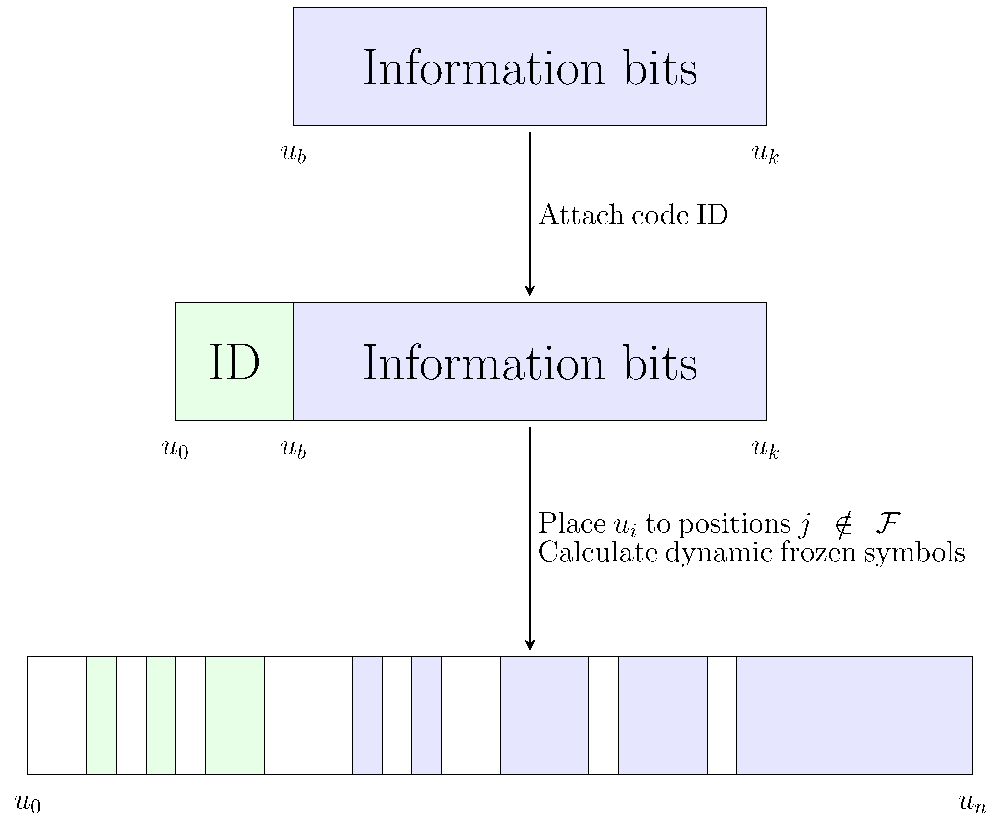
\includegraphics[width=0.45\textwidth]{./pictures/BlindStructure.eps}
  }\qquad
  \subfloat[Правая картинка]{
    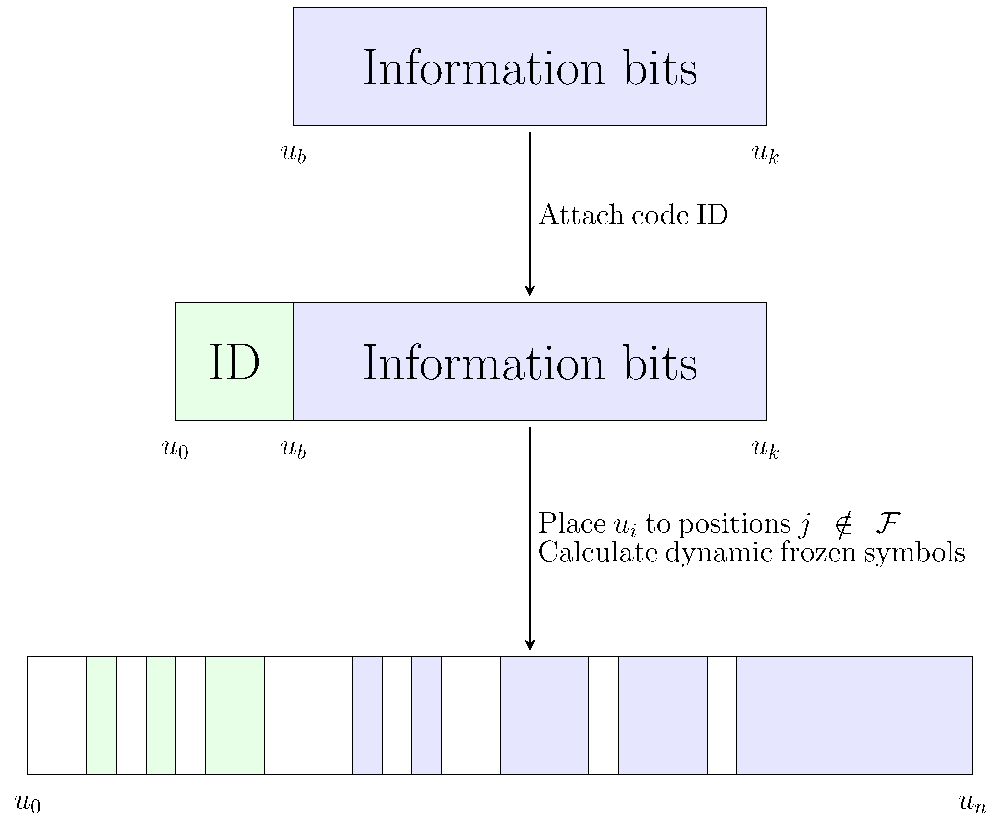
\includegraphics[width=0.45\textwidth]{./pictures/BlindStructure.eps}
  }
  \caption{Две одинаковых картинки}
  \label{2figs}
\end{figure}

%----------------------------------------------------------------------------------------
\subsection{hyperref, url}
Пакеты позволяют вставлять интерактивные ссылки в документ.
Примеры: 
\url{https://en.wikibooks.org/wiki/LaTeX/Hyperlinks},
\hyperlink{contents}{\contentsname}.

%----------------------------------------------------------------------------------------
\subsection{algorithm2e}
Пакет предоставляет вставлять в документ псевдокод алгоритмов.
В документе представлен алгоритм \ref{IR}.
% there is algorithm, function and procedure environments
\begin{procedure}
  % do not print semicolon at the end of each line
  \DontPrintSemicolon

  % define keywords, describing input and output parameters
  \SetKwInOut{Input}{input}
  \SetKwInOut{Output}{output}

  % describe variables
  \SetKwData{Left}{left}
  \SetKwData{This}{this}
  \SetKwData{Up}{up}

  % describe functions
  \SetKwFunction{Union}{Union}
  \SetKwFunction{FindCompress}{FindCompress}

  % begin of the algorithm description
  \Input{A bitmap $Im$ of size $w\times l$}
  \Output{A partition of the bitmap}
  \BlankLine

  \emph{текст на русском}\;
  еще текст на русском\;
  $i \leftarrow 2$\;
  \While{$i < l$}{
    \emph{special treatment of the first element of line $i$}\;
    \For{$j \leftarrow 2$ \KwTo $w$}{\label{forins}
      \Left $\leftarrow$ \FindCompress{$Im[i,j-1]$}\;
      \Up $\leftarrow$ \FindCompress{$Im[i-1,]$}\;
      \This $\leftarrow$ \FindCompress{$Im[i,j]$}\;

      \If(\tcp*[h]{O(\Left,\This)==1}){\Left compatible with \This}{\label{lt}
        \lIf{\Left $<$ \This}{\Union{\Left,\This}}
        \lElse{\Union{\This,\Left}}
      }

      \If(\tcp*[f]{O(\Up,\This)==1}){\Up compatible with \This}{\label{ut}
        \lIf{\Up $<$ \This}{\Union{\Up,\This}}
        \tcp{\This is put under \Up to keep tree as flat as possible}\label{cmt}
        \lElse{\Union{\This,\Up}}\tcp*[h]{\This linked to \Up}\label{lelse}
      }
    }
    \lForEach{element $e$ of the line $i$}{\FindCompress{p}}
  }

  \caption{IntervalRestriction($Im$)}
  \label{IR}
\end{procedure}


%----------------------------------------------------------------------------------------
\subsection{listings}
Пакет позволяет вставлять в текст листинги кода.
Пример кода C++ приведен на листинге \ref{l1}.

\begin{minipage}{\linewidth} % prevent page break inside listing
\begin{lstlisting}[caption={Hello,world!},label=l1]
  #include <iostream>
  int main() {
    std::cout << ``Hello, world!'' << std::endl;
    return 0;
  }
\end{lstlisting}
\end{minipage}

%----------------------------------------------------------------------------------------
\section{todonotes}
Пакет позволяет вставлять комментарии в документ, которые могут служить напоминанием при разработке большого документа.
\todo{Вставить ссылку}

Список всех комментариев может быть сформирован командой {\em listoftodos}.
\todo[inline]{Написать еще текста}

%----------------------------------------------------------------------------------------
%       BIBLIOGRAPHY
%----------------------------------------------------------------------------------------
\clearpage
\printbibliography

\listoftodos[TODO notes]
\end{document}


